\section{Using Ground Temperatures with Basements}\label{using-ground-temperatures-with-basements}

The basement routine is used to calculate the face (surface) temperatures on the outside of the basement wall or the floor slab. This is the plane between the outside insulation and the basement wall. The insulation thermal resistance can range from zero (no insulation) to any reasonable value. The units are K/(W/m\(^{2}\)). The program will simulate two conditions: full insulation from grade to the footing or half insulation that extends halfway down from grade to footing. The temperature on this plane is used with the OtherSideCoefficients object in EnergyPlus to supply the outside face temperature of the walls or slab.

\begin{figure}[hbtp] % fig 22
\centering
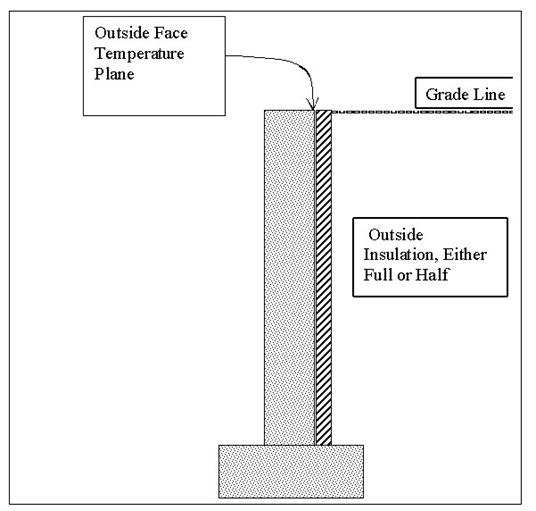
\includegraphics[width=0.9\textwidth, height=0.9\textheight, keepaspectratio=true]{media/image020.jpg}
\caption{Basement Configuration \protect \label{fig:basement-configuration}}
\end{figure}

The output from the program is a csv file, named MonthlyResults.csv, as shown below.

\begin{figure}[hbtp] % fig 23
\centering
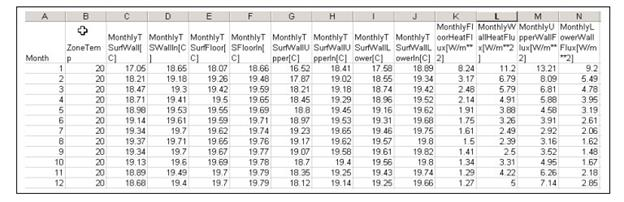
\includegraphics[width=0.9\textwidth, height=0.9\textheight, keepaspectratio=true]{media/image021.jpg}
\caption{Output from Basement program \protect \label{fig:output-from-basement-program}}
\end{figure}

Column B gives the basement zone temperature. This can vary month by month as will be explained later. Column C is the monthly average wall outside face temperature, as shown in the diagram above. Column D is the corresponding average monthly average inside wall face temperature. Columns E and F contain the same information for the basement floor slab. Columns G-J contain the same information for the upper half and the lower half of the basement walls.

Columns K through N contain the monthly average heat flux for the floor, the walls, the upper half of the walls and the lower half of the walls. The flux is reported in units of W/m\(^{2}\).

The program also produces an output file named EPObjects.TXT. This file contains the necessary idf objects to make it easy to include the wall outside surface temperatures in an EnergyPlus input file. Idf objects for all of the temperatures in the output file shown above are included. These objects are explained in detail in the section Using the Interface Surface Temperature Results in EnergyPlus.
